\documentclass[a4paper,11pt]{article}

\usepackage[spanish]{babel}
\usepackage[utf8]{inputenc}

\usepackage{amsmath}
\usepackage{siunitx}

\usepackage{graphicx}
\usepackage{float}
\usepackage[font=small,labelfont=bf]{caption}
\usepackage[colorlinks=true]{hyperref}


\title{Preinforme: Caracterización de componentes electrónicos utilizando una placa de audio}
\date{\today}
\author{Micaela Toscani, Axel Lacapmesure y Guillermo Brinatti}

\begin{document}
\maketitle

\section{Introducción}

El objetivo de este trabajo consiste en describir la curva de respuesta de un diodo y la característica de un elemento integrado. Para ello utilizamos una placa de sonido de computadora como generador de ondas y como placa de adquisición, alimentando los diversos circuitos con su salida de audio y registrando la señal deseada con su entrada. En la sección \ref{sec:metodo} describimos la instrumentación de nuestro trabajo, particularizando en \ref{sec:biblioteca} sobre la implementación del control de la placa de sonido mediante una biblioteca programada en Python y en \ref{sec:caracterizacion} sobre la caracterización de la placa de audio como generador de ondas y placa de adquisición. A continuación dedicamos la sección \ref{sec:resultados} a la caracterización de los componentes elegidos, donde en \ref{sec:discreto} mostramos y discutimos los resultados obtenidos en la medición de la respuesta del diodo, mientras que en \ref{sec:integrado} presentamos la propuesta de trabajo para la caracterización de un componente integrado.

\section{Método}
\label{sec:metodo}

	\subsection{Biblioteca utilizada}
	\label{sec:biblioteca}
	% Descripción biblioteca pyaudio e implementación en el código de los callbacks
	
	El control de la placa de sonido fue llevado a cabo a partir de programar una biblioteca propia en lenguaje Python que incluya las funciones orientadas al usuario final necesarias para utilizar el dispositivo como generador de ondas y placa de adquisición \cite{repo}. Para ello nos basamos en la biblioteca \emph{\href{https://people.csail.mit.edu/hubert/pyaudio/}{PyAudio}} \cite{pyaudio}, la cual consiste en una implementación de alto nivel y en Python de la API multiplataforma provista en C/C++ por \emph{\href{http://www.portaudio.com/}{PortAudio}} \cite{portaudio}.
	
	La comunicación con la placa de sonido se basa en el paradigma de \emph{callbacks} de entrada y salida, que consiste en funciones que se ejecutan en bucles concurrentes y realizan respectivamente la lectura y escritura de los \emph{buffers} que el sistema operativo dispone para el dispositivo para grabar y reproducir audio. En la implementación de nuestra librería, cada función \emph{callback} cuenta con un \emph{buffer} circular propio tipo FIFO (\emph{first input, first output}) que alojan la señal que se quiere emitir (en el caso del \emph{callback} de salida) y la señal que se está registrando (en el caso del \emph{callback} de entrada). En cada iteración de ambos bucles se transfiere un paquete de datos de tamaño fijo y configurable que se guarda en el correspondiente \emph{buffer} de forma cíclica, permitiendo una ejecución continua similar a la obtenida en un generador de funciones y un osciloscopio, donde las interrupciones en la ejecución debido a problemas de latencia pueden ser evitadas ajustando debidamente los tamaños del paquete y del \emph{buffer}.

	La figura \ref{fig:flowchart} muestra el diagrama de flujo de un proceso de emisión y adquisición de señales con la placa de audio. La primera etapa comprende la inicialización de los parámetros de funcionamiento y la generación de las señales de salida a partir de una función que sintetiza y guarda en la memoria señales con formas de onda típicas cuyas características (amplitud, frecuencia, etc.) son configurables. En esta etapa además se emplean funciones auxiliares para calibrar la señales a unidades de tensión y para multiplexar los canales en orden de poder trabajar con dos canales (modo estéreo de la placa de audio). En la sección \ref{sec:caracterizacion} describiremos los análisis que nos permitieron desarrollar estas funciones. Posteriormente se prealoja la memoria de los \emph{buffers} y se inicializan los contadores y variables auxiliares necesarias para el funcionamiento de los \emph{callbacks}. Posteriormente se inicia el proceso de lectura y escritura abriendo los flujos de datos y desencadenando la ejecución concurrente de los bucles de lectura y escritura. El programa espera hasta la finalización de ambos flujos una vez que se alcanza el límite de datos transferidos establecido, momento en el cual se procede a cerrar los flujos de lectura y escritura y a demultiplexar y calibrar las señales adquiridas de forma análoga a lo realizado con las señales emitidas.
	
    \begin{figure}[!h] 
        \centering
        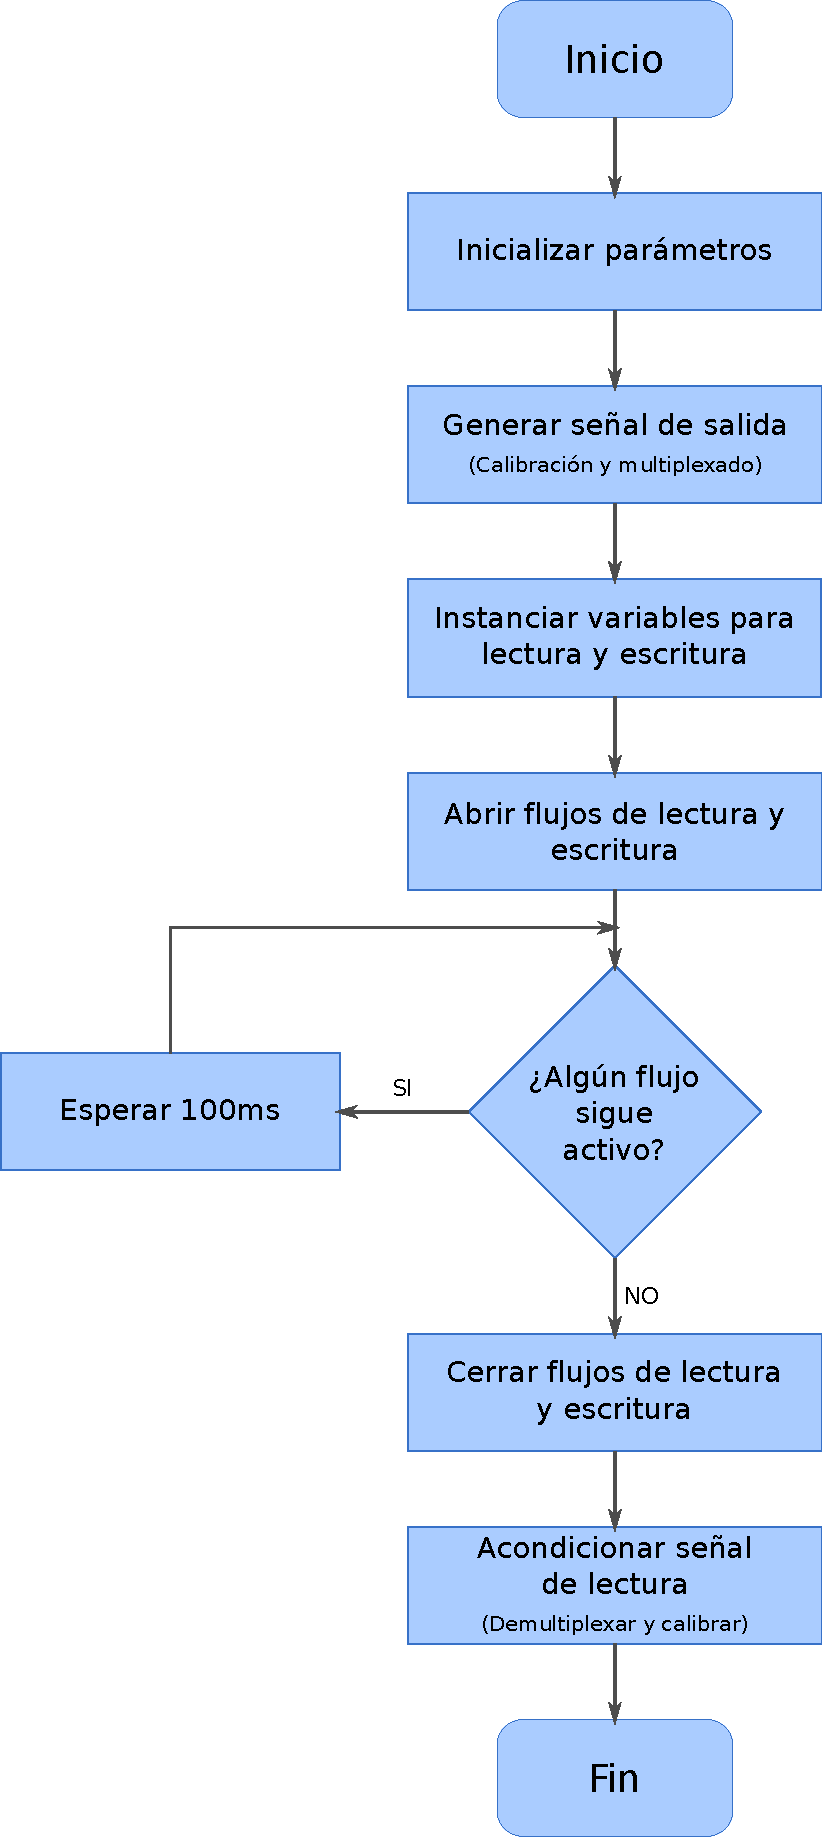
\includegraphics[width=0.7\textwidth]{imagenes/flowchart.pdf}
        \caption{Diagrama de flujo.
        }
        \label{fig:flowchart}
 
    \end{figure}
    \clearpage
	
	\subsection{Caracterización placa de sonido}
	\label{sec:caracterizacion}
    % Respuesta en frecuencia (amplitud, fase), piso de ruido,
    % linealidad, problemática de tirar los puntos iniciales, gráfico
    % para describir multiplexado/demulitiplexado

En el presente trabajo utilizamos la placa de sonido \emph{Realtek
"MODELO"} para generación y adquisición de señales.  Para ello
utilizamos el puerto de salida analógica estéreo principal y el puerto
de entrada analógica estéreo \emph{line-in}, respectivamente.

Al adquirir señales estéreo con la placa de sonido, esta multiplexa las
señales de los dos canales en un mismo paquete de datos. En la
\textbf{Figura} \ref{fig:multiplexado} se muestra el paquete de datos
obtenido al ingresar una señal senoidal por uno de los canales de
entrada mientras el otro canal se encuentra conectado a
GND.
Para poder separar las dos señales adquiridas en modo estéro se
implementó una función de demultiplexado que permite manipular por
separado las señales de ambos canales de entrada.  Del mismo modo que
con la señal de entrada, cuando se desea utilizar ambos canales de la
salida estéreo se debe proveer a la placa de sonido un paquete de datos
con las dos señales multiplexadas. Para facilitar la manipulación de esos
datos también implementamos la función de multiplexado respectiva.

    \begin{figure}[!h] 
        \centering
        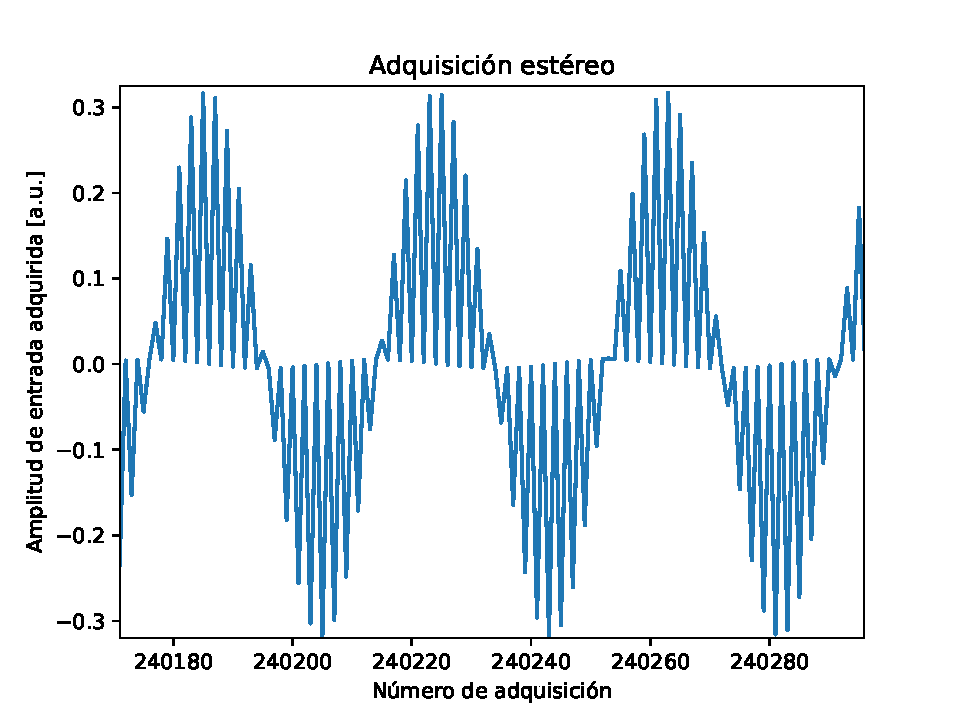
\includegraphics[width=0.9\textwidth]{imagenes/estereo.pdf}
        \caption{Paquete de datos obtenidos al leer la señal de entrada
estereo cuando un canal se encuentra alimentado por una señal senoidal
mientras el otro canal se encuentra conectado a GND.}
        \label{fig:multiplexado} 
    \end{figure}

Los paquetes de datos que se reciben y se envían a la placa de sonido
contienen la información de la amplitud de las señal traducida a una
unidad de cuentas aribtraria. Para poder establecer la correlación de
esta unidad arbitraria con un valor de tensión realizamos un proceso de
calibración tanto de la entrada como de la salida de la placa de sonido.
Para ello generamos con la placa de sonido señales sinusoidales de
distintas amplitudes, estas señales fueron medidas con un osciloscopio
externo y a su vez fueron ingresadas como entrada a la placa de sonido.
Se registraron los valores de las unidades arbitrarias y su valores de
tensión respectivo con el objetivo de ajustar una curva de calibración
tanto de los canales de entrada como de los canales de salida de la
placa.  En las \textbf{Figuras} \ref{fig:CalibracionEntrada} y
\ref{fig:CalibracionSalida} se muestran las curvas de calibración
obtenidas.  Los datos medidos fueron ajustados linealmente obteniéndose
las siguientes expresiones,
	
\begin{equation*}
	 \text{Tensión de salida} = \SI{1.620}{\V} \times Cuentas% + \SI{0.1080}{\V}
\end{equation*}

\begin{equation*}
	\text{Tensión de entrada} = \SI{2.555}{\V} \times Cuentas% + \SI{0.09116}{\V}
\end{equation*}

Utilizando las curvas de calibración obtenidas generamos funciones
adicionales que permiten convertir una señal que contiene la información
en cuentas de unidad arbitraria en valores de tensión y viceversa.

	\begin{figure}[!h]
		\centering
		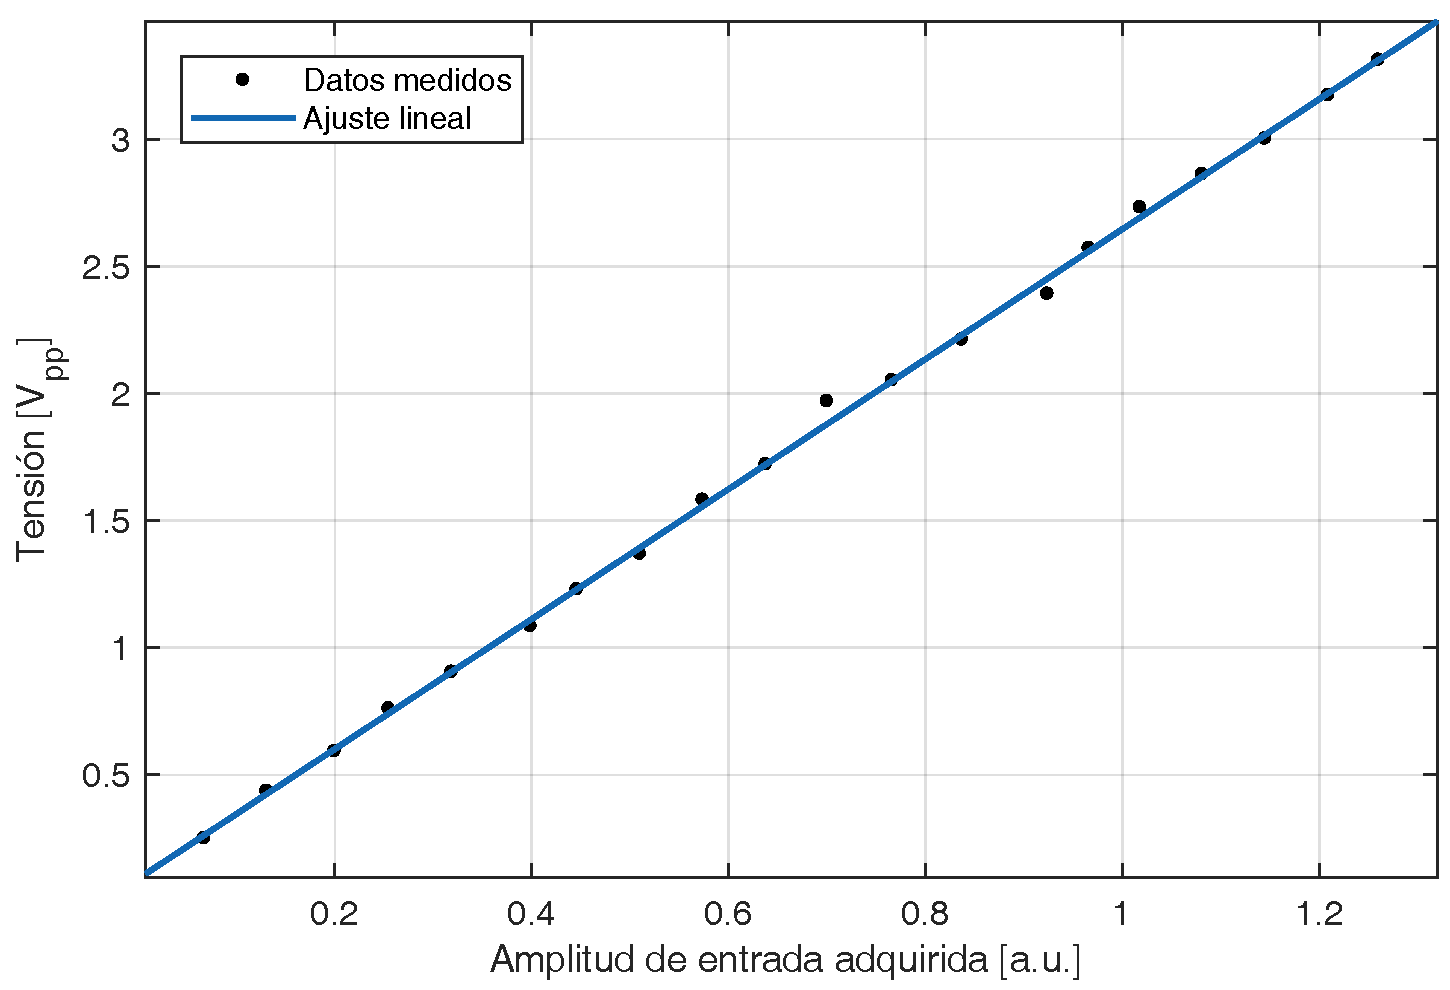
\includegraphics[width=\textwidth]{imagenes/CalibracionEntrada.pdf}
		\caption{Curva de calibración de la señal de entrada de la placa
de sonido.}
        \label{fig:CalibracionEntrada}
	\end{figure}
	
	\begin{figure}[!h]
		\centering
		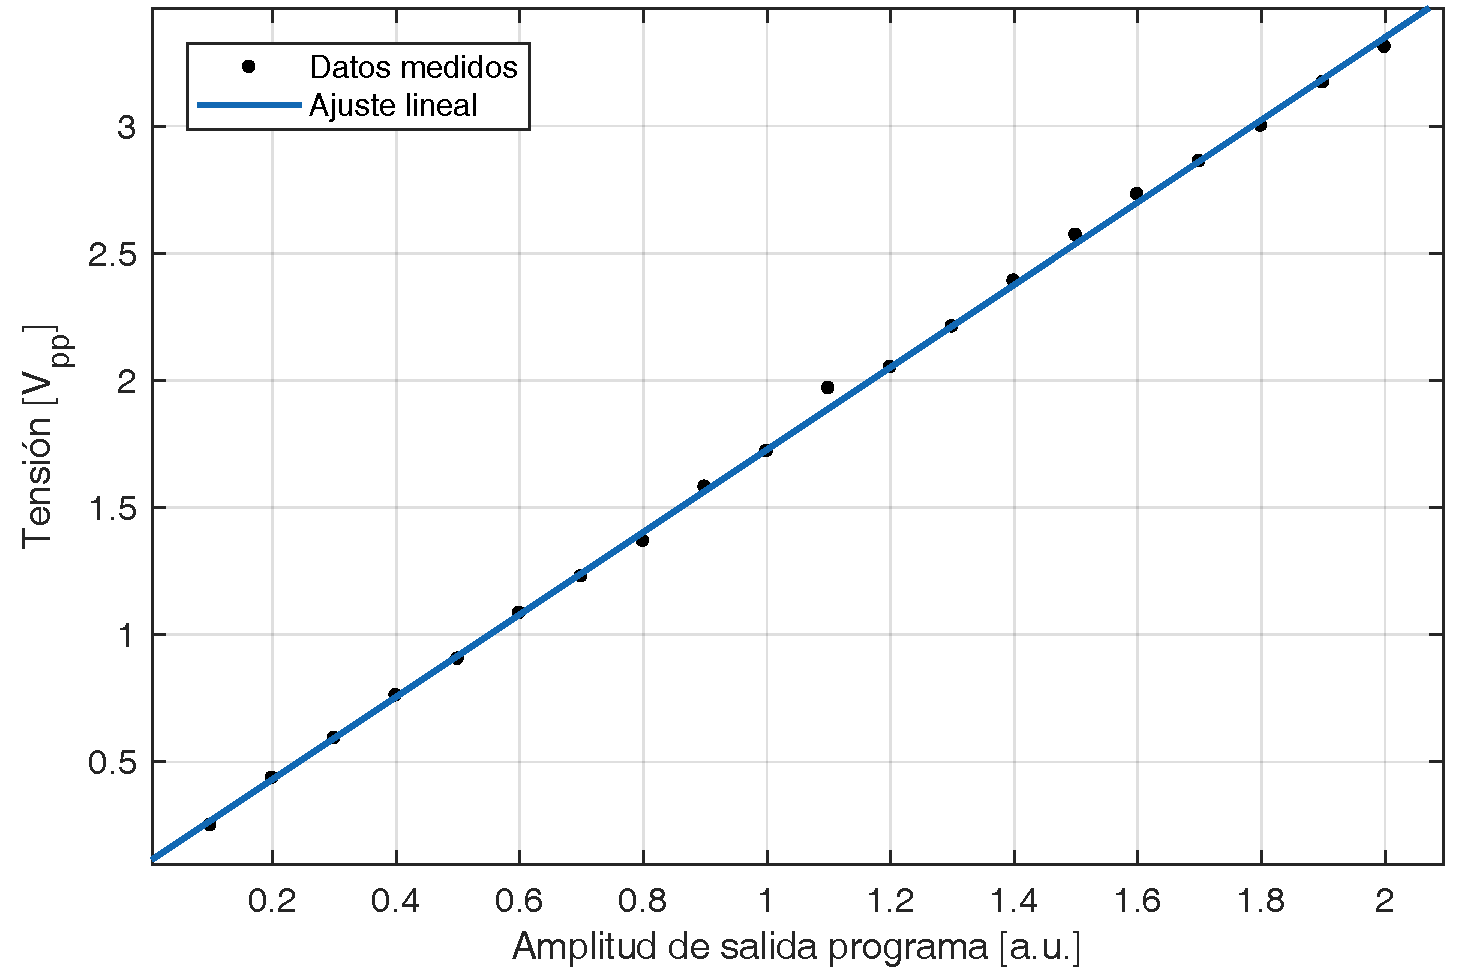
\includegraphics[width=\textwidth]{imagenes/CalibracionSalida.pdf}
		\caption{Curva de calibración de la señal de salida de la placa
de sonido.}
        \label{fig:CalibracionSalida}
	\end{figure}

Para poder caracterizar la respuesta en frencuencia de la placa de
sonido realizamos un barrido en frecuencias generando señales
sinusoidales de distintas frecuencias con la salida de la placa que
fueron ingresada como entrada a la misma. Registramos la variación en la
respuesta del sistema en función de la frecuencia, los resultados se
muestran en las \textbf{Figuras} \ref{fig:bode44k1} y \ref{fig:bode192k}
para dos frecuencias de muestreo distintas.

	\begin{figure}[!h]
		\centering
		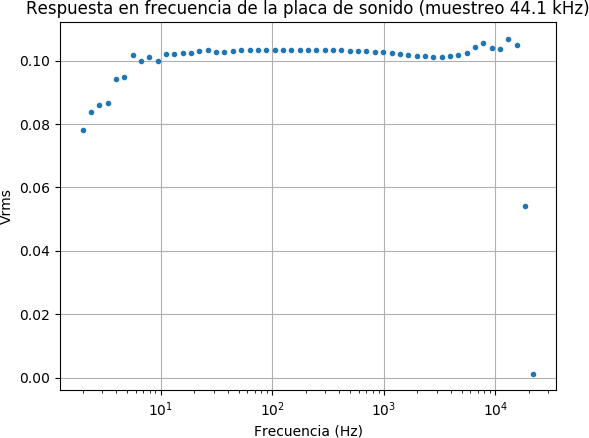
\includegraphics[width=0.9\textwidth]{imagenes/bode44k1Hz.png}
		\caption{Variación de la ganancia en función de la frecuencia de
la señal, para una frecuencia de muestreo configurada de \SI{44.1}{\kHz}}
        \label{fig:bode44k1}
	\end{figure}

	\begin{figure}[!h]
		\centering
		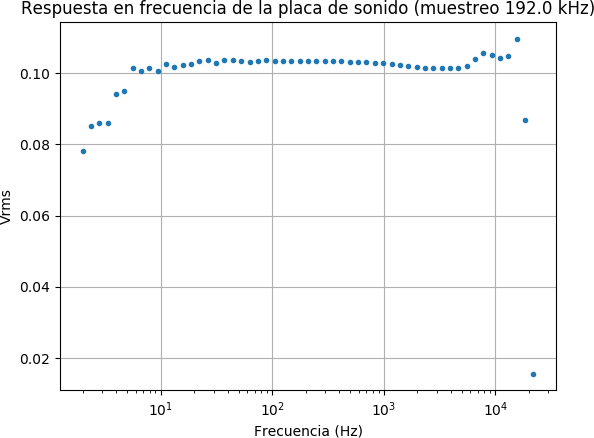
\includegraphics[width=0.9\textwidth]{imagenes/bode192kHz.png}
		\caption{Variación de la ganancia en función de la frecuencia de
la señal, para una frecuencia de muestreo configurada de \SI{192}{\kHz}}
        \label{fig:bode192k}
	\end{figure}

Para poder establecer el mínimo valor de señal de tensión que puede
registrarse con la placa de sonido medimos el piso de rudio de la misma.
Conectamos ambos canales de la entrada estéreo a GND y registramos la
señal obtenida, los resultados para cada canal se muestran en las
\textbf{Figuras} \ref{fig:RuidoIzquierdo} y \ref{fig:RuidoDerecho}.
El valor del rudio RMS obtenido es de $\SI{277}{\uV}$. En las mismas figuras puede verse además como, aproximadamente, los primeros \SI{300}{\milli\second} de cada adquisición son ceros. Este tiempo de espera inicial se encontró siempre y no depende fuertemente de los parámetros con los que se define la adquisición. Esto parece indicar que esta latencia entre el momento en que la placa empieza a enviar datos al buffer y el momento en el que comienza realmente la adquisición es característico de la misma y no puede evitarse. De esta forma, todas las mediciones mostradas en este trabajo descartan esos primeros \SI{300}{\milli\second} de medición de manera de conservar solo la información relevante en cada experimento.  

	\begin{figure}[h]
		\centering
		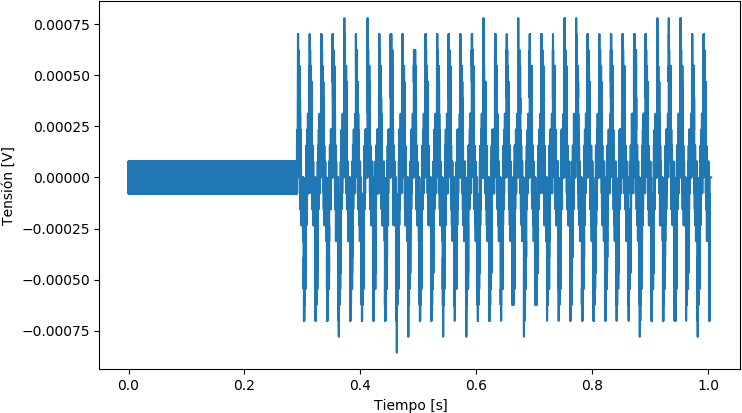
\includegraphics[width=0.9\textwidth]{imagenes/RuidoCanalIzquierdo.png}
		\caption{Señal de ruido correspondiente al canal izquierdo del
puerto de entrada estéreo.}
        \label{fig:RuidoIzquierdo}
	\end{figure}
	
	\begin{figure}[h]
		\centering
		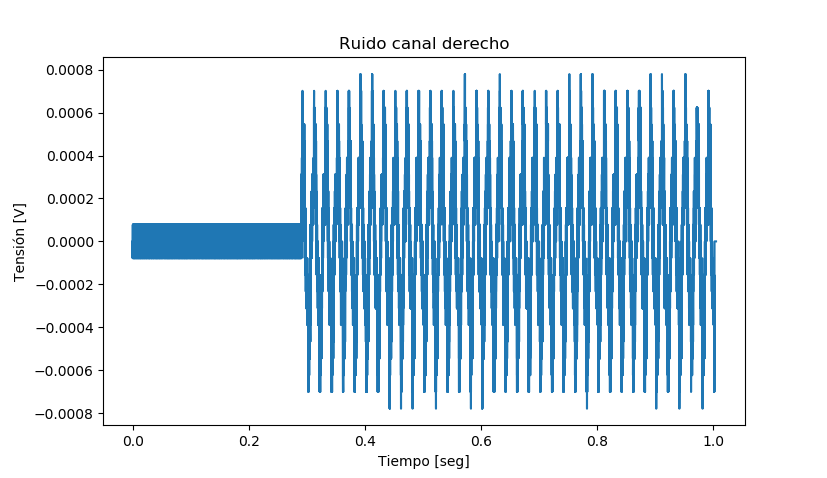
\includegraphics[width=0.9\textwidth]{imagenes/RuidoCanalDerecho.png}
		\caption{Señal de ruido correspondiente al canal derecho del
puerto de entrada estéreo.}
        \label{fig:RuidoDerecho}
	\end{figure}
\clearpage

\section{Resultados}
\label{sec:resultados}

En esta sección se describiran los resultados de las caracterizaciones de los componentes electrónicos utilizando la placa de sonido tanto como dispositivo de adquisición como generador de funciones. 
	\subsection{Componente discreto: Diodo 1N4148}
	\label{sec:discreto}
	Se caracterizó la curva de corriente en función de la caida de tensión en un diodo rápido modelo 1N4148. Para esto se utilizó uno de los canales de salida de la placa como fuente de tensión. La misma se conectó en serie con el diodo a estudiar y una resistencia de carga de \SI{100}{\ohm}. La señal elegida fue una señal sinusoidal de frecuencia \SI{1}{\kilo\hertz} y amplitud 2 Vpp (máxima permitida por el dispositivo). La adquisición se realizó a dos canales, donde el primero se utilizó para medir la fuente y el segundo para la caída en el diodo. A partir de la diferencia entre estas mediciones se calculó la caída de tensión en la resistencia y luego la corriente. Con estos datos se realizó el gráfico que se muestra en la figura \ref{fig:diodo}, donde se muestra el resultado final de la caracterización. Cabe destacar que la placa de adquisición posee un filtro pasa altos en la entrada, por lo que el valor de continua de la medición se pierde en ambos canales. Esto es un problema para la medición de la caída en el diodo pues la misma no tiene valor medio cero. Esta es una limitación de la placa utilizada y no puede ser corregida sin información o hipótesis adicionales. En nuestro caso, basta con asumir que la corriente será cero cuando la fuente está apagada.   
	
	\begin{figure}[h]
		\centering
		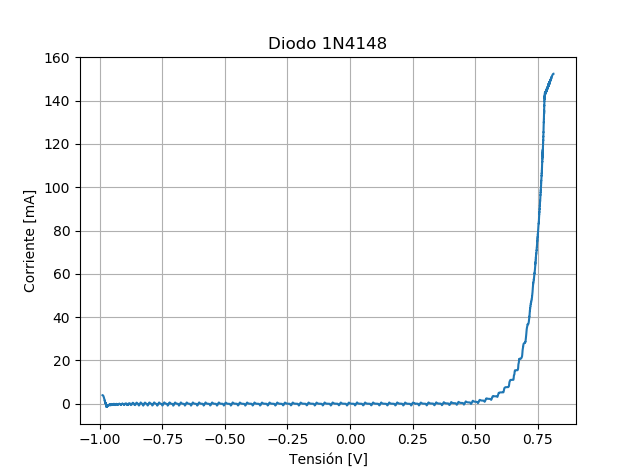
\includegraphics[width=\textwidth]{imagenes/Diodo1N4148.png}
		\caption{Curva de corriente en función de la tensión para un diodo 1N4148 caracterizada utilizando la placa de sonido tanto como fuente de tensión como placa de adquisición.}
		\label{fig:diodo}
	\end{figure}
	
	\subsection{Integrado}	\label{sec:integrado}
	
	La caracterización del componente integrado quedó pendiente. Para esta se propone caracterizar el rechazo de ripple en un regulador LM317. Para esto, se plantea armar el circuito mostrado en la figura \ref{fig:lm317}. En este se plantea adquirir el ripple de la señal de entrada y el de la señal de salida utilizando ambos canales de la placa. Como es deseable utilizar una fuente con ripple controlable, se plantea el uso de un generador de funciones externo ya que se necesita una señal con valor medio distinto de cero. Otra posibilidad a investigar es la de adicionar al circuito lo necesario para sumar a las salidas de la placa (utilizadas para generar el ripple) una fuente de continua que de un valor medio a la señal.
		
	\begin{figure}[h]
		\centering
		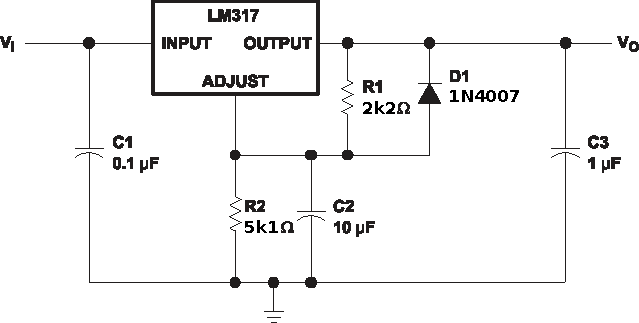
\includegraphics[width=\textwidth]{imagenes/lm317.pdf}
		\caption{Circuito propuesto para la caracterización del rechazo de ripple en un integrado LM317.}
		\label{fig:lm317}
	\end{figure}

\clearpage

\begin{thebibliography}{99}

	\bibitem{repo} Repositorio en GitHub de la biblioteca propia utilizada en el trabajo, \href{https://github.com/fotonicaOrg/placadeaudio}{URL: https://github.com/fotonicaOrg/placadeaudio}, actualizado el 19/09/2018. La biblioteca está programada en el archivo \emph{PlacaAudio.py}.
	\bibitem{pyaudio} Página web oficial de PyAudio, \href{https://people.csail.mit.edu/hubert/pyaudio/}{URL: https://people.csail.mit.edu/hubert/pyaudio/}, accedido el 19/09/2018.
	\bibitem{portaudio} Página web oficial de PortAudio, \href{http://www.portaudio.com/}{URL: http://www.portaudio.com/}, accedido el 19/09/2018.
	
	\bibitem{datasheetlm317} Hoja de datos del regulador LM317 proporcionada por Texas Instruments.  \href{http://www.ti.com/lit/ds/symlink/lm317.pdf}{URL: http://www.ti.com/lit/ds/symlink/lm317.pdf}

\end{thebibliography}



\end{document}
